\subsection{Data Generator and Compare}
\label{sect:bg-blocks-data-generator-and-compare-block}
Data can come from the instruction register or the data generator.  A mux select signal is generated based on the current operation.  For user data patterns, the data from the instruction register is selected and written to memory.  For NPSF patterns, the data generator outputs the word to be written to memory.  The comparator checks if the data read from memory matches what is expected and generates the pass/fail signal.

\subsubsection{Data Generator}
\begin{figure}[h!]
  \centering
  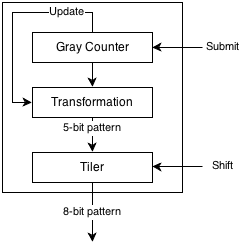
\includegraphics[scale=0.5]{datagen}
  \caption{Data Generator Block Diagram}
  \label{fig:datagen}
\end{figure}
The data generator block design is shown in \ref{fig:datagen}.  The gray counter is a 5-bit counter that generates gray code and repeats after 32 iterations.  The gray code is passed to the transform block which converts the code to a Eulerian Sequence.  A detailed description of the Euler Sequence can be found in \cite{1675556}.  Essentially, a 5-bit Euler Sequence used as the Type-1 NPSF background will transition through all the possible read and write combinations that could occur.  This requires 161 different sequences which can be broken into five groupings as shown in \ref{tab:euler}.  Except for the first column, each column is generated by a one-bit right shift and rotate followed by inverting the most and least significant bits \cite{00957583}.

\begin{table}[h]
  \caption{Partial 5-bit Euler Sequence}
  \centering
  \begin{tabular}{c c c c c c}
  \hline\hline
  Iteration    & Gray (E[0]) & E[1]  & E[2]  & E[3]  & E[4]  \\
  X0  & 00000 & 10001 & 01001 & 00101 & 00011 \\
  X1  & 00001 & 00001 & 00001 & 00001 & 00001 \\
  X2  & 00011 & 00000 & 10001 & 01001 & 00101 \\
  ......             & ...   & ...   & ...   & ...   & ...   \\
  X29 & 10011 & 01000 & 10101 & 01011 & 00100 \\
  X30 & 10001 & 01001 & 00101 & 00011 & 00000 \\
  X31 & 10000 & 11001 & 01101 & 00111 & 00010 \\ [0.5ex]
  \end{tabular}
  \label{tab:euler}
\end{table}

The transformation block provides the 5-bit Euler Sequence to be used as the NPSF background.  To write this value to memory using the Type-1 tiling method, the sequence must be spread over the adjacent rows to create the correct tiling background as shown in \ref{fig:tiling}.  

\begin{figure}[h!]
  \centering
  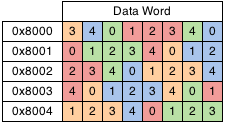
\includegraphics[scale=0.5]{type1tiling}
  \caption[Type-1 Neighborhood Tiling Method for Design]{Type-1 Neighborhood Tiling Method for Design}  
   Each 5-bit color block represents one Type-1 neighborhood.
  \label{fig:tiling}
\end{figure}

\subsubsection{Data Comparator}
Each read march element is checked with the data comparator.  The comparator accepts as inputs the TDS bus and the output of the MUT.  If the MUT output matches the TDS value, a pass signal is generated.  If there is any discrepancy, the fail signal is generated.  

\subsubsection{Polarity and Data Register}
The polarity signal from the current march operation is used to invert the data.  If the polarity signal is false (0), the data is unmodified and stored to the data register.  If the polarity signal is true (1), the data is inverted, then stored in the data register.  


